% !TeX spellcheck = en_GB
% !TeX program = xelatex
\documentclass{report}

% we have to load xcolor first, see http://tex.stackexchange.com/questions/99049/latex-error-option-clash-for-package-xcolor-even-if-i-put-listings-before
\usepackage[dvipsnames]{xcolor}

% thanks to http://tex.stackexchange.com/a/47579/71109
\usepackage{ifxetex}
\usepackage{ifluatex}
\newif\ifxetexorluatex % a new conditional starts as false
\ifnum 0\ifxetex 1\fi\ifluatex 1\fi>0
   \xetexorluatextrue
\fi

\ifxetexorluatex
  \usepackage{fontspec}
\else
  \usepackage[T1]{fontenc}
  \usepackage[utf8]{inputenc}
%  \usepackage[lighttt]{lmodern}
\fi

\usepackage{amsmath}
\usepackage{amssymb}
\usepackage{etoolbox}
\usepackage{xspace}
\newtoggle{textualoperators}

\usepackage{tikz}
% Using the forest package, there is a known issue that edges sometimes cut through child nodes.
% See the package documentation on CTAN (https://www.ctan.org/pkg/forest), section 6.2. "Known bugs", "Edges cutting through sibling nodes":
% While it would be possible to fix the situation after child alignment (at least for some child alignment methods), I have decided against that, since the distances between siblings would soon become too large. [...] The bottomline is, please use manual adjustment to fix such situations.
\usepackage{forest}

\tikzset{every node/.style={draw}}

\newcommand{\lxor}{\oplus}

\newcommand{\tuple}[1]{\langle #1 \rangle}
\newcommand{\concatenation}{\Vert}

\newcommand{\literal}[1]{\mathsf{#1}}
\newcommand{\atom}[1]{\mathsf{#1}}

\newcommand{\var}[1]{\mathtt{#1}}
\newcommand{\edgevariable}[2]{\left[\var{#1}
	\ifstrempty{#2}{}{\colon{\atom{#2}}}
	\right]}
\newcommand{\nodevariable}[2]{(\var{#1}
	\ifstrempty{#2}{}{\colon{\atom{#2}}}
	)}

% alpha operators

\newcommand{\expandbody}[3]{~_{\nodevariable{#1}{}}^{\nodevariable{#2}{#3}}}

% see http://tug.ctan.org/info/symbols/comprehensive/symbols-a4.pdf
\newcommand{\expandop}{\updownarrow}
\newcommand{\expand}[5]{\expandop \edgevariable{#1}{#2} \expandbody{#3}{#4}{#5}}

\newcommand{\expandoutop}{\uparrow}
\newcommand{\expandout}[5]{\expandoutop \edgevariable{#1}{#2} \expandbody{#3}{#4}{#5}}

\newcommand{\expandinop}{\downarrow}
\newcommand{\expandin}[5]{\expandinop \edgevariable{#1}{#2} \expandbody{#3}{#4}{#5}}

\newcommand{\getverticesop}{\bigcirc}
\newcommand{\getvertices}[2]{\getverticesop_{\nodevariable{#1}{#2}}}

\newcommand{\getedgesop}{\mathbin{\text{\rotatebox[origin=c]{90}{$\multimapboth$}}}}
\newcommand{\getedges}[6]{\getedgesop_{\nodevariable{#1}{#2}}^{\nodevariable{#3}{#4}} \edgevariable{#5}{#6}}

\newcommand{\alldifferentop}{\neq}
\newcommand{\alldifferent}[1]{\alldifferentop_{\atom{#1}}}

\newcommand{\duplicateeliminationop}{\delta}
\newcommand{\duplicateelimination}{\duplicateeliminationop}

\newcommand{\sortop}{\tau}
\newcommand{\sortopasc}{\tau^\Uparrow}
\newcommand{\sortopdesc}{\tau^\Downarrow}

\newcommand{\sortarbitrary}[3]{\sortop^{#1}_{#2}{#3}}

\newcommand{\sort}[2]{\sortop_{#1}{#2}}
\newcommand{\sortasc}[2]{\sortopasc_{#1}{#2}}
\newcommand{\sortdesc}[2]{\sortopdesc_{#1}{#2}}

\newcommand{\projectionop}{\pi}
\newcommand{\projection}[1]{\projectionop_{#1}}

\newcommand{\selectionop}{\sigma}
\newcommand{\selection}[1]{\selectionop_{\atom{#1}}}

\newcommand{\renameop}{\rho}
\newcommand{\rename}[1]{\renameop_{#1}}

\newcommand{\groupingop}{\gamma}
\newcommand{\grouping}[1]{\groupingop_{#1}}

\newcommand{\topop}{\lambda}
\newcommand{\topp}[2]{\topop_{#1}^{#2}}
\newcommand{\skipp}[1]{\topop^{#1}}
\newcommand{\limit}[1]{\topop_{#1}}

% beta operators

\newcommand{\joinop}{\bowtie}
\newcommand{\join}{\joinop}

\newcommand{\leftouterjoinop}{\leftouterjoin}
\newcommand{\myleftouterjoin}{\leftouterjoinop}

\newcommand{\antijoinop}{\, \triangleright \,}
\newcommand{\antijoin}{\antijoinop}

\newcommand{\unionop}{\cup}
\newcommand{\union}{\unionop}

\newcommand{\bagunionop}{\uplus}
\newcommand{\bagunion}{\bagunionop}

\newcommand{\minusop}{\setminus}
\newcommand{\minus}{\minusop}

\newcommand{\intersectionop}{\cap}
\newcommand{\intersection}{\intersectionop}

\newcommand{\cartesianproductop}{\times}
\newcommand{\cartesianproduct}{\cartesianproduct}


%\usepackage[a4paper,top=2cm,bottom=2cm,left=2cm,right=2cm]{geometry}
\usepackage[a4paper,margin=2.5cm]{geometry}
\usepackage{hyperref}

\usepackage{graphicx}
\usepackage{fancyhdr}
\usepackage{csquotes}
\usepackage{microtype}
\usepackage[math]{blindtext}
\usepackage{url}
\usepackage{booktabs}
\usepackage{multirow}
\usepackage{array}
\usepackage{rotate}
\usepackage{enumitem}
\usepackage{todonotes}
\usepackage{adjustbox}
\usepackage{autobreak}
\usepackage{xstring}
\usepackage{progressbar}
\usepackage{lineno}
\usepackage{accsupp}
\usepackage{datetime}
%\usepackage{tocstyle} % prevents numbers an titles from overlapping in ToC

\renewcommand{\thelinenumber}{
	\BeginAccSupp{ActualText={}}\arabic{linenumber}\EndAccSupp{}%
}

\pagestyle{fancy}
\fancyhf{}

\renewcommand{\subsectionmark}[1]{\def\subsectiontitle{: #1}}
\fancyhead[L]{\nouppercase{\rightmark}} % \StrLeft{\subsectiontitle}{50}}}
\fancyhead[R]{\thepage}

\renewcommand{\figureautorefname}{Figure}
\renewcommand{\tableautorefname}{Table}
\renewcommand{\partautorefname}{Part}
\renewcommand{\chapterautorefname}{Chapter}
\renewcommand{\sectionautorefname}{Section}
\renewcommand{\subsectionautorefname}{Section}
\renewcommand{\subsubsectionautorefname}{Section}

\newcommand{\retescale}{0.45}
\newcommand{\patternscale}{0.28}
\newcommand{\diagramscale}{0.75}
\newcommand{\phasesscale}{0.5}

\newcommand{\mysf}[1]{$\mathsf{#1}$}
\newcommand{\query}[1]{\mysf{#1}\xspace}

\newcommand{\connectedsegments}{\query{ConnectedSegments}}
\newcommand{\poslength}{\query{PosLength}}
\newcommand{\routesensor}{\query{RouteSensor}}
\newcommand{\switchmonitored}{\query{SwitchMonitored}}
\newcommand{\switchset}{\query{SwitchSet}}
\newcommand{\semaphoreneighbor}{\query{SemaphoreNeighbor}}

\newcommand{\iq}{\mbox{\textsc{IncQuery}}\xspace}
\newcommand{\iqd}{\mbox{\textsc{IncQuery-D}}\xspace}
\newcommand{\eiq}{\mbox{\textsc{EMF-IncQuery}}\xspace}
\newcommand{\viatraquery}{\mbox{\textsc{Viatra} Query}\xspace}
\newcommand{\vql}{\mbox{\textsc{Viatra} Query Language}\xspace}
\newcommand{\tb}{Train Benchmark\xspace}
\newcommand{\antlr}{\mbox{ANTLR4}\xspace}
\newcommand{\saphana}{SAP \mbox{HANA}\xspace}
\newcommand{\ingraph}{\textsf{ingraph}\xspace}
\newcommand{\opencypher}{\mbox{openCypher}\xspace}
\newcommand{\cypher}{\mbox{Cypher}\xspace}
\newcommand{\sparql}{\mbox{SPARQL}\xspace}
\newcommand{\rga}{relational graph algebra\xspace}
\newcommand{\RGA}{Relational Graph Algebra\xspace}

\newcommand{\queryplanscale}{0.9}

\newcommand{\fig}[4]{
	\centerline{\includegraphics[scale=#4]{#1}}
	\captionof{figure}{#3.}\label{fig:#2}
}

\newcommand{\queryplan}[2]{\fig{../ingraph/visualization/#1.pdf}{#1}{#2}{\queryplanscale}}

\newcommand{\eg}{e.g.\xspace}
\newcommand{\ie}{i.e.\xspace}
\newcommand{\etal}{et al.\xspace}
\newcommand{\wrt}{w.r.t.\xspace}

% text for operators
\newcommand{\operatortext}[1]{\mbox{\emph{#1}}\xspace}

\newcommand{\projectiontext}{\operatortext{projection}}
\newcommand{\selectiontext}{\operatortext{selection}}
\newcommand{\antijointext}{\operatortext{antijoin}}
\newcommand{\jointext}{\operatortext{natural join}}
\newcommand{\leftouterjointext}{\operatortext{left outer join}}
\newcommand{\cartesianproducttext}{\operatortext{Cartesian product}}
\newcommand{\uniontext}{\operatortext{union}}
\newcommand{\baguniontext}{\operatortext{bag union}}
\newcommand{\intersectiontext}{\operatortext{intersection}}
\newcommand{\minustext}{\operatortext{minus}}
\newcommand{\renametext}{\operatortext{rename}}

\newcommand{\alldifferenttext}{\operatortext{all-different}}
\newcommand{\duplicateeliminationtext}{\operatortext{duplicate-elimination}}
\newcommand{\sorttext}{\operatortext{sorting}}
\newcommand{\groupingtext}{\operatortext{grouping}}
\newcommand{\toptext}{\operatortext{top}}
\newcommand{\unwindtext}{\operatortext{unwind}}

\newcommand{\expandouttext}{\operatortext{expand-out}}
\newcommand{\expandintext}{\operatortext{expand-in}}
\newcommand{\expandbothtext}{\operatortext{expand-both}}

\newcommand{\getverticestext}{\operatortext{get-vertices}}
\newcommand{\getedgestext}{\operatortext{get-edges}}

\newcommand{\yes}{$\mdlgblkcircle$\xspace}
\newcommand{\no}{$\mdlgwhtcircle$\xspace}

\newcommand{\append}{\,\|\,}
\newcommand{\appendtext}{\operatortext{append}}
\newcommand{\remove}{-}
\newcommand{\removetext}{\operatortext{remove}}

\newcommand{\breakable}[2][c]{%
	\begin{tabular}[#1]{@{}l@{}}#2\end{tabular}}

\newcommand{\vertexlabels}{L_v}
\newcommand{\edgelabels}{L_e}

\newcommand{\verticestoedges}{\mathsf{src\_trg}}
\newcommand{\propertyfunction}[2]{\mathrm{#1}(#2)}

\newcommand{\vertexproperties}{P_v}
\newcommand{\edgeproperties}{P_e}

\newcommand{\vertexproperty}[1]{p_{#1}}
\newcommand{\edgeproperty}[1]{p_{#1}}

\newcommand{\vertexlabelfunction}{l_v}
\newcommand{\edgelabelfunction}{l_e}

\newcommand{\assign}{\rightarrow}

\newcommand{\attr}[1]{\mathrm{attr}(#1)}
\newcommand{\dom}[1]{\mathrm{dom}(#1)}
\newcommand{\schema}[1]{\mathrm{sch}(\mathsf{#1})}

%\newcommand{\relnull}{\bot}
%\newcommand{\relnull}{-}
\newcommand{\relnull}{\varepsilon}
\newcommand{\bigunion}{\bigcup}
\newcommand{\op}[2]{\mathrm{#1}\left(#2\right)}

%if lstlistings is used
%better approach: use the minted package - see https://en.wikibooks.org/wiki/LaTeX/Source_Code_Listings#The_minted_package
%SzG: updating minted is quite cumbersome, see http://tex.stackexchange.com/questions/18083/how-to-add-custom-c-keywords-to-be-recognized-by-minted
\usepackage{listings}

\definecolor{lightgray}{RGB}{242,242,242}
\definecolor{keywordcolor}{RGB}{0,0,160}
\definecolor{commentcolor}{RGB}{0,128,64}
\definecolor{stringcolor}{RGB}{0,128,0}
\lstset{
	numbers=left,
	numberstyle=\scriptsize\ttfamily,
	stepnumber=1,
	numbersep=5pt,
	%
	backgroundcolor=\color{lightgray},
	basicstyle=\scriptsize\ttfamily, % print whole listing small
	keywordstyle=\color{keywordcolor}\bfseries\ttfamily,
	commentstyle=\color{commentcolor}\ttfamily,
	stringstyle=\color{stringcolor}\ttfamily,
	identifierstyle=, % nothing happens
	%
	showstringspaces=false, % no special string spaces
	aboveskip=3pt,
	belowskip=3pt,
	columns=flexible,
	keepspaces=true,
	breaklines=true,	
	frameround=tttt,
	captionpos=b,
	frame=tb,
	framerule=0pt,
	framexleftmargin=0.25em,
	tabsize=4,
}

\lstdefinelanguage{cypher}
{
	morekeywords={
		MATCH, OPTIONAL, WHERE, NOT, AND, OR, XOR, RETURN, DISTINCT, ORDER, BY, ASC, ASCENDING, DESC, DESCENDING, UNWIND, AS, UNION, WITH, ALL, CREATE, DELETE, DETACH, REMOVE, SET, MERGE, SET, SKIP, LIMIT,
		% some legacy rules
		INDEX, DROP, UNIQUE, CONSTRAINT, EXPLAIN, PROFILE, START, CASE,
		% some SQL-only keywords
		GROUP,
	},
	sensitive=true,
	morecomment=[l]{//},
	morecomment=[s]{/*}{*/},
	morestring=[b]{"},
}

\lstset{language=Cypher}


\nonfrenchspacing

% title page
\title{openCypher Specification}
\author{G\'abor Sz\'arnyas, J\'ozsef Marton}

\begin{document}

\begin{titlepage}
	\begin{center}
		
\includegraphics[width=60mm,keepaspectratio]{figures/bme-logo}\\
		\vspace{0.3cm}
		\textbf{Budapest University of Technology and Economics}\\
		\textmd{Faculty of Electrical Engineering and Informatics}\\[5cm]

		\vspace{0.4cm}
		{\huge \bfseries Formalisation of openCypher Queries in Relational Algebra (Extended Version)}\\[0.8cm]
		\vspace{0.5cm}
		\textsc{\Large Technical Report}\\[4cm]

		{\Large Gábor Szárnyas, József Marton}\\

		\IfFileExists{./disable-appendix}{}{
			\vspace{2cm}
			\begin{tabular}{llr@{ of }l}
			\input{appendix/progressbar-tck}
			\input{appendix/progressbar-fraud-detection}
			\input{appendix/progressbar-ldbc-snb-interactive}
			\input{appendix/progressbar-ldbc-snb-bi}
			\input{appendix/progressbar-movie-database}
			\input{appendix/progressbar-static-analysis-java}
			\input{appendix/progressbar-static-analysis-javascript}
			\input{appendix/progressbar-trainbenchmark}
			\input{appendix/progressbar-adbis-examples}
			\input{appendix/progressbar-cikm-examples}
			\input{appendix/progressbar-railway-verification}
			\end{tabular}
		}

		\vfill

		\IfFileExists{./commit-message}{
			{\large Commit: \texttt{\input{commit-message}}}
		}{}
	\end{center}
\end{titlepage}

% this is the simplest way to count the title page in the page numbers, while not displaying the page number on the title page
\addtocounter{page}{1}


\tableofcontents

% !TeX spellcheck = en_GB
% !TeX encoding = UTF-8
\chapter*{Executive Summary}
\label{chp:executive-summary}

This document is generated on each commit of the \ingraph repository\footnote{\url{https://github.com/FTSRG/ingraph}}.

\paragraph{Structure.} \autoref{chp:foundations} introduces the theoretical foundations of the \opencypher language. \autoref{chp:incremental} presents incremental relational operators.

\paragraph{Appendices.} The appendix chapters contain sets of Cypher queries, and their representations as relational algebraic expressions and trees, along with their incremental equivalents.

\begin{itemize}
	\item \autoref{chp:tck}: the acceptance tests defined in the \opencypher Technology Compliance Kit\footnote{\url{https://github.com/opencypher/openCypher/tree/master/tck}}.
	\item \autoref{chp:fraud-detection}: fraud detection queries based on the Neo4j white paper.
	\item \autoref{chp:ldbc-snb-interactive}: LDBC Social Network Benchmark's Interactive queries.
  \item \autoref{chp:ldbc-snb-bi}: LDBC Social Network Benchmark's BI queries.
	\item \autoref{chp:movie-database}: Movie Database queries from the Neo4j tutorials.
	\item \autoref{chp:static-analysis-java}: Java static analysis queries.
	\item \autoref{chp:static-analysis-javascript}: JavaScript static analysis queries.
	\item \autoref{chp:trainbenchmark}: Train Benchmark queries.
\end{itemize}


\chapter{Theoretical Foundations}
\label{chp:foundations}

\graphicspath{{./figures/}}

\section{Introduction}
\label{sec:introduction}

%https://markorodriguez.com/2013/01/09/on-graph-computing/

\paragraph{Context.} Graphs are a well-known formalism, widely used for describing and analysing systems. Graphs provide an intuitive formalism for modelling real-world scenarios, as the human mind tends to interpret the world in terms of objects (\emph{vertices}) and their respective relationships to one another (\emph{edges})~\cite{CollectivelyGeneratedModel}. 

The \emph{property graph} data model~\cite{DBLP:books/igi/Sakr11/RodriguezN11} extends graphs by adding labels and properties for both vertices and edges. This gives a rich set of features for users to model their specific domain in a natural way. Graph databases are able to store property graphs and query their contents with complex graph patterns, which, otherwise would be are cumbersome to define and/or inefficient to evaluate on traditional relational databases and query technologies.

Neo4j~\cite{Neo4j}, a popular NoSQL property graph database, offers the Cypher~\cite{Cypher} query language to specify graph patterns. Cypher is a high-level declarative query language which can be optimised by the query engine. The \opencypher project~\cite{openCypher} is an initiative of Neo Technology, the company behind Neo4j, to deliver an open specification of Cypher.

\paragraph{Problem and objectives.} The \opencypher project features a formal specification of the grammar of the query language (\autoref{sec:opencypher}) and a set of acceptance tests that define the behaviour of various Cypher features. However, there is no mathematical formalisation for any of the language features. In ambiguous cases, the user is advised to consult Neo4j's Cypher documentation or to experiment with Neo4j's Cypher query engine and follow its behaviour. Our goal is to provide a formal specification for the core features of \opencypher.

\paragraph{Contributions.} In this paper, we use a formal definition of the property graph data model~\cite{DBLP:conf/edbt/HolschG16} and an extended version of relational algebra, operating on multisets (bags) and featuring additional operators~\cite{DBLP:books/daglib/0020812}. These allow us to construct a concise formal specification for the core features in the \opencypher grammar, which can then serve as a basis for implementing an \opencypher-compliant query engine.


\section{Preliminaries}
\label{sec:preliminaries}

This section defines the mathematical concepts used in the paper. Our notation closely follows~\cite{DBLP:conf/edbt/HolschG16} and is similar to~\cite{DBLP:books/igi/Sakr11/RodriguezN11}\footnote{The formalism presented in~\cite{DBLP:books/igi/Sakr11/RodriguezN11} lacks the notion of \emph{vertex labels}.}.

\subsection{Property Graph Data Model}

A \emph{property graph} is defined as $G = (V, E, \verticestoedges, \vertexlabels, \edgelabels, \vertexlabelfunction, \edgelabelfunction, \vertexproperties, \edgeproperties)$, where $V$ is a set of vertices, $E$ is a set of directed edges, $\verticestoedges: E \assign V \cartesianproductop V$ assigns the source and target vertices to edges. The graph is labelled (or typed):
\begin{itemize}
	\item $\vertexlabels$ is a set of vertex labels, $\vertexlabelfunction: V \assign 2^{\vertexlabels}$ assigns \emph{a set of labels} to each vertex.
	\item $\edgelabels$ is a set of edge labels, $\edgelabelfunction: E \assign \edgelabels$ assigns \emph{a single label} to each edge.
\end{itemize}

Furthermore, graph $G$ has properties (\emph{attributed graph}). Let $D$ be a set of atomic domains.
\begin{itemize}
	\item $\vertexproperties$ is a set of vertex properties. A vertex property $p_i \in \vertexproperties$ is a function $p_i: V \assign D_i \unionop \{ \relnull \}$, which assigns a property value from a domain $D_i \in D$ to a vertex $v \in V$, if $v$ has property $p_i$, otherwise $p_i(v)$ returns $\relnull$.
	\item $\edgeproperties$ is a set of edge properties. An edge property $p_j \in \edgeproperties$ is a function $p_j: E \assign D_j \unionop \{ \relnull \}$, which assigns a property value from a domain $D_j \in D$ to an edge $e \in E$, if $e$ has property $p_j$, otherwise $p_j(e)$ returns $\relnull$.
\end{itemize}

\paragraph{Running example.} \autoref{fig:running-example-property-graph} presents an example inspired by the Movie Database dataset\footnote{\url{https://neo4j.com/developer/movie-database/}}.

\begin{minipage}[b]{0.48\linewidth}
	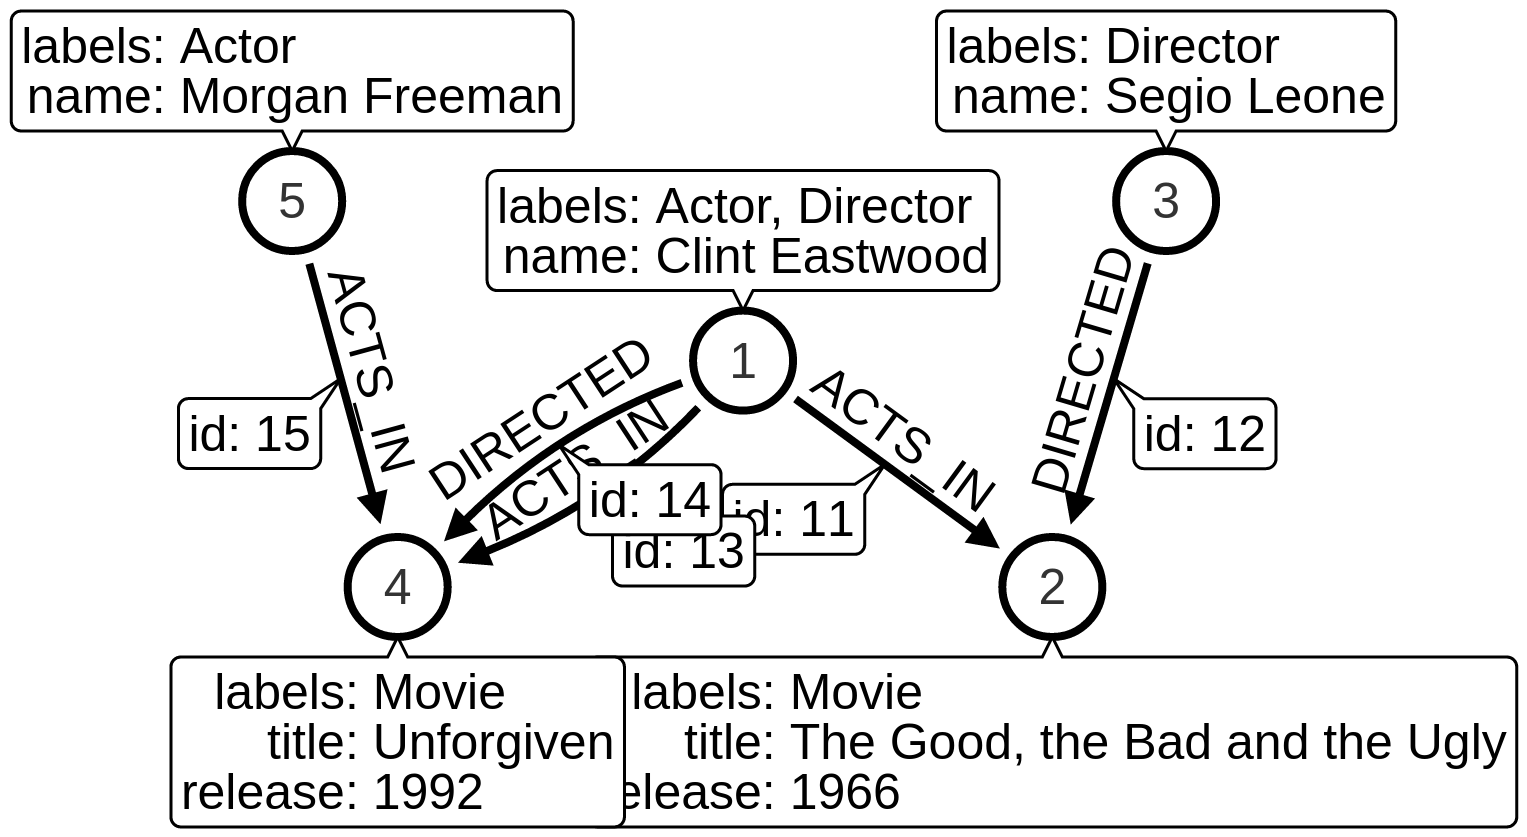
\includegraphics[width=6cm]{movie-graph}
	\captionof{figure}{Example movie graph.}
	\label{fig:running-example-property-graph}
\end{minipage}
\begin{minipage}[b]{0.53\linewidth}
	\footnotesize
	$V=\{1, 2, 3, 4, 5\}; E=\{11,12,13,14,15\};$
	
	$\verticestoedges(11) = \tuple{1, 2}; \verticestoedges(12) = \tuple{3, 2}; \ldots$

	$\vertexlabels = \{\atom{Actor}, \atom{Director}, \atom{Movie}\};$

	$\edgelabels = \{\atom{ACTS\_IN}, \atom{DIRECTED}\};$

	$\vertexlabelfunction(1) = \{\atom{Actor}, \atom{Director}\}; \vertexlabelfunction(2) = \{\atom{Movie}\}; \ldots;$

	$\edgelabelfunction(11) = \atom{ACTS\_IN}; \edgelabelfunction(12) = \atom{DIRECTED}; \ldots;$

	$\vertexproperties = \{\atom{name}, \atom{title}, \atom{release}\}; \edgeproperties = \{\};$

	$\propertyfunction{name}{1} = \atom{'Clint~Eastwood'}; \propertyfunction{name}{2} = \relnull; \ldots$

	$\propertyfunction{title}{1} = \relnull; \propertyfunction{title}{2} = \atom{'The~Good,~the~Bad~and~the~Ugly'}; \ldots$
	
	$\propertyfunction{release}{1} = \relnull; \propertyfunction{release}{2} = \atom{1966}; \ldots$
	\captionof{figure}{The dataset represented as a property graph.}
	\label{fig:property-graph-formalized}
\end{minipage}

In the context of this paper, we define a \emph{relation} as a bag (\emph{multiset}) of tuples: a tuple can occur more than once in the relation~\cite{DBLP:books/daglib/0020812}.
Given a property graph $G$, relation $r$ is a \emph{graph relation} if the following holds:
$$\forall A \in \attr{r}: \dom{A} \subseteq V \union E \union D,$$
where $\attr{r}$ is the set of attributes of $r$, $\dom{A}$ is the domain of attribute $A$. The schema of $r$, $\schema{r}$ is a list containing the attribute names. For schema transformations, the \appendtext operator is denoted by $\append$, the \removetext operator is denoted by $\remove$.

\subsection{Foundations of Relational Algebra}

\paragraph{Basic operators of relational algebra.} We give a brief summary of the operators in relational algebra. A more detailed discussion is available in database textbooks, \eg~\cite{DBLP:books/daglib/0006733}.

\paragraph{Unary operators.} The \projectiontext operator $\projectionop$ keeps a specific set of attributes in the relation: $ t = \projection{A_1, \ldots, A_n} \left(r\right).$ Note that the tuples are not deduplicated by default, \ie the results will have the same number of tuples as the input relation $r$. The projection operator can also rename the attributes, \eg $\projection{v1 \assign v2} \left(r\right)$ renames $\atom{v1}$ to $\atom{v2}$.
The \selectiontext operator $\selectionop$ filters the incoming relation according to some criteria. Formally,
$ t = \selection{\theta} \left(r\right), $
where predicate $\theta$ is a propositional formula. The operator selects all tuples in $r$ for which $\theta$ holds.

\paragraph{Binary operators.} The $\unionop$ operator produces the set union of two relations, while the $\bagunionop$ operator produces the \emph{bag union} of two operators, \eg $\{\tuple{1, 2}, \tuple{1, 2}, \tuple{3, 4}\} \bagunionop \{\tuple{1, 2}\} = \{\tuple{1, 2}, \tuple{1, 2}, \tuple{1, 2}, \tuple{3, 4}\}$. For both the \uniontext and \baguniontext operators, the schema of the operands must have the same number of attributes. Some authors also require that they share a common schema, \ie have the same set of attributes~\cite{DBLP:books/daglib/0020812}.

The $\cartesianproductop$ operator produces the \cartesianproducttext:

$$ t = r \cartesianproductop s.$$

The result of the \jointext operator $\joinop$ is determined by creating the Cartesian product of the relations, then filtering those tuples which are equal on the attributes that share a common name. The combined tuples are projected: from the attributes present in both of the two input relations, we only keep the ones in $r$ and drop the ones in $s$. Thus, the join operator is defined as
$$r \join s = \pi_{R \union S} \left(\selection{r.A_1 = s.A_1\,\land\,\ldots\,\land\,r.A_n = s.A_n)} \left(r \times s\right) \right),$$
where $ \{ A_1, \ldots, A_n \} $ is the set of attributes that occur both in $R$ and $S$, \ie $ R \intersection S = \{ A_1, \ldots, A_n \} $. Note that if the set of common attributes is empty, the \jointext operator is equivalent to the Cartesian product of the relations.
The join operator is both commutative and associative: $r \join s = s \join r$ and $(r \join s) \join t = r \join (s \join t)$, respectively.

The \antijointext operator $\antijoinop$ (also known as \emph{left anti semijoin}) collects the tuples from the left relation $r$ which have no matching pair in the right relation $s$:
$$ t = r \antijoin s = r \setminus \pi_{R} \left(r \join s\right), $$
where $\pi_{R}$ denotes a projection operator, which only keeps the attributes of the schema over relation $r$. The antijoin operator is not commutative and not associative.

The \leftouterjointext $\myleftouterjoin$ pads tuples from the left relation that did not match any from the right relation with $\relnull$ values and adds them to the result of the \jointext~\cite{DBLP:books/daglib/0015084}:
$$ t = r \myleftouterjoin s = (r \join s) \union (r \antijoin s) \cartesianproductop \{\relnull, \ldots, \relnull\}, $$

where the constant relation $\{\relnull, \ldots, \relnull\}$ is on the schema $S \setminus R$.

\subsection{Common Extensions to Relational Algebra}

Most textbooks also define \emph{extended operators} of relational algebra~\cite{DBLP:books/daglib/0020812}:

\begin{itemize}
	\item The \duplicateeliminationtext operator $\duplicateeliminationop$ eliminates duplicate tuples in a bag.
	\item The \groupingtext operator $\groupingop$ groups tuples according to their value in one or more attributes and aggregates the remaining attributes. %Aggregated values (scalars and inline collections) makes \rga not closed under \groupingtext.
	\item The \sorttext operator $\sortop$ transforms a bag relation of tuples to a list of tuples by ordering them. The ordering is defined by specified attributes of the tuples with an ordering direction (ascending $\asc$/descending $\desc$) for each attribute, \eg $\sortop_{\asc \atom{v1}, \desc \atom{v2}} (r)$.
\end{itemize}

The \toptext operator $\topp{l}{s}$ (adapted from~\cite{DBLP:conf/sigmod/LiCIS05}) takes a list as its input, skips the top $s$ tuples and returns the next $l$ tuples.\footnote{SQL implementations offer the \texttt{OFFSET} and the \texttt{LIMIT}/\texttt{TOP} keywords.}

\subsection{Graph-Specific Extensions to Relational Algebra}
\label{sec:rga}

We adapted graph-specific operators from~\cite{DBLP:conf/edbt/HolschG16}\footnote{The \textsc{GetNodes} operator introduced in~\cite{DBLP:conf/edbt/HolschG16} and did not support labels. We extended it by allowing the specification of vertex labels and renamed it to \getverticestext to be consistent with the rest of the definitions. We also extended the \textsc{ExpandIn} and \textsc{ExpandOut} operators to allow it to return a set of edges, and introduced the \expandbothtext operator to allow navigation to both directions.} and propose an additional operator.

The \getverticestext nullary operator $\getvertices{v}{t_1 \land \ldots \land t_n}$ returns a graph relation of a single attribute $v$ that contains the ID of all vertices that have \emph{all} of labels $t_1, \ldots, t_n$.

The \expandbothtext unary operator $\expandboth{E}{l_1 \lor \ldots \lor l_k \ast min \ldots max}{v}{w}{t_1 \land \ldots \land t_n}(r)$ adds (1)~a new attribute $w$ to $r$ containing the IDs of vertices having \emph{all} labels $t_1, \ldots, t_n$ that can be reached from vertices of attribute $v$ by traversing edges having \emph{any} labels $l_1, \ldots, l_n$, and (2)~a new attribute $E$ for the edges of the path from $v$ to $w$. The operator may use at least $\atom{min}$ and at most $\atom{max}$ hops, both defaulting to $1$ if omitted. % With the default setting, \ie $\atom{min}=\atom{max}=1$, a single edge variable $e$ can be used instead of edge list $E$.
The \expandintext operator~$\expandinop$ and \expandouttext operator~$\expandoutop$ only consider directed paths from $w$ to $v$ and from $v$ to $w$, respectively.

We propose the \alldifferenttext operator to guarantee the uniqueness of edges (see the remark on \emph{uniqueness of edges} in \autoref{sec:opencypher}). The \alldifferenttext operator $\alldifferent{E_1, E_2, E_3, \ldots}{(r)}$ filters $r$ to keep tuples where the variables in $\bigcup_{i} E_{i}$ are pairwise different.\footnote{Should e.g. $E_2$ be a set of the single variable $e_2$, the variable name can be used as a shorthand instead, so $\alldifferent{E_1, e_2, E_3, \ldots}{(r)} ~ \equiv ~ \alldifferent{E_1, \{e_2\}, E_3, \ldots}{(r)}$}
It can be expressed as a \selectiontext:
$$\alldifferent{E_1, E_2, E_3, \ldots}{(r)} = \selection{ \bigwedge\limits_{e_1, e_2 \,\in\, \bigcup\limits_{i} {E_i} ~ \wedge ~ { e_1 \,\neq\, e_2 } } { r.e_1 \,\neq\, r.e_2 } }{(r)}$$

\paragraph{Property access.} Assuming that $x$ is an attribute of a graph relation, we use the notation $x.a$ in (1)~attribute lists for projections and (2)~selection conditions to express the access to the corresponding value of property $a$ in the property graph~\cite{DBLP:conf/edbt/HolschG16}.

\paragraph{Summary.} \autoref{table:collections} provides an overview of the operators of \rga.

\newcommand{\propheader}{\multirow{2}{*}{\bf prop.}}
\newcommand{\rgaheader}{\multirow{2}{*}{\breakable{\bf RGA}}}

\setlength\tabcolsep{3.6pt}
\begin{table}[htb]
	\centering
	\begin{tabular}{||c||c|c|c||c|c|c||c||c||}
		\hline
		\multirow{2}{*}{\bf ops} &             \multirow{2}{*}{\bf operator}             &         \multirow{2}{*}{\bf name}         & \propheader & \multicolumn{3}{c||}{\bf output for} &             \multirow{2}{*}{\bf schema}              \\ \cline{5-7}
		&                                                       &                                           &             & \bf set & \bf bag &     \bf list     &  \\ \hline\hline
		\multirow{1}{*}{\bf 0}   &                  $\getvertices{v}{}$                  &             \getverticestext              &     set     &   set   &   set   &       set        &                  $\tuple{\atom{v}}$                  \\ \hline\hline %\cline{2-8}
%		&              $\getedges{v}{}{w}{}{e}{}$               &               \getedgestext               &     $-$     &   $-$   &   $-$   &       $-$        &               $\tuple{\atom{v, e, w}}$               \\ \hline\hline
		\multirow{8}{*}{\bf 1}   &         $\projection{v_1, v_2, \ldots} (r)$         &              \projectiontext              &      i      &   bag   &   bag   &       list       &         $\tuple{\atom{v_1, v_2, \ldots}}$          \\ \cline{2-8}
		&              $\selection{condition} (r)$              &              \selectiontext               &      i      &   set   &   bag   &       list       &                     $\schema{r}$                     \\ \cline{2-8}
		&            $\expandboth{v}{w}{}{e}{} (r)$             &              \expandbothtext              &     $-$     &   set   &   bag   &       list       &       $\schema{r} \append \tuple{\atom{e, w}}$       \\ \cline{2-8}
		&            $\alldifferent{variables} (r)$             &             \alldifferenttext             &      i      &   set   &   bag   &       list       &                     $\schema{r}$                     \\ \cline{2-8}
		&             $\duplicateeliminationop (r)$             &         \duplicateeliminationtext         &      i      &   set   &   set   &       list       &                     $\schema{r}$                     \\ \cline{2-8}
		&                     $\sort{\desc \atom{v_1}, \asc \atom{v_2}, \ldots} (r)$                     &                 \sorttext                 &      i      &  list   &  list   &       list       &                     $\schema{r}$                     \\ \cline{2-8}
		&          $\grouping{v_1, v_2, \ldots} (r)$          &               \groupingtext               &      i      &   set   &   set   &       set        &         $\tuple{\atom{v_1, v_2, \ldots}}$          \\ \cline{2-8}
		&                     $\topop (r)$                      &                 \toptext                  &     $-$     &  list   &  list   &       list       &                     $\schema{r}$                     \\ \hline\hline
		\multirow{5}{*}{\bf 2}   & $r \unionop s$, $r \minusop s$ & \uniontext, \minustext &     $-$     &   set   &   set   &       set        &                     $\schema{r}$                     \\ \cline{2-8}
		&                    $r \bagunion s$                    &               \baguniontext               &    c, a     &   bag   &   bag   &       bag        &                     $\schema{r}$                     \\ \cline{2-8}
		&               $r \cartesianproductop s$               &           \cartesianproducttext           &    c, a     &   set   &   bag   &       bag        &           $\schema{r} \append \schema{s}$            \\ \cline{2-8}
		&                    $r \joinop s$                      &                 \jointext                 &    c, a     &   set   &   bag   &       bag        & $\schema{r} \append (\schema{s} \minus \schema{r}) $ \\ \cline{2-8}
		&                $r \myleftouterjoin s$                 &            \leftouterjointext             &     $-$     &   set   &   bag   &       bag        & $\schema{r} \append (\schema{s} \minus \schema{r}) $ \\ \cline{2-8}
		&                   $r \antijoinop s$                   &               \antijointext               &    c, a     &   set   &   bag   &       bag        &                     $\schema{r}$                     \\ \cline{1-8}
	\end{tabular}
	\caption{Properties of relational graph algebra operators. A unary operator $\alpha$ is idempotent~(i), iff $\alpha(x) = \alpha(\alpha(x))$ for all inputs. A binary operator $\beta$ is commutative~(c), iff $x~\beta~y = y~\beta~x$ and associative~(a), iff $(x~\beta~y)~\beta~z = x~\beta~(y~\beta~z)$.}
	\label{table:collections}
\end{table}


\section{The openCypher Query Language}
\label{sec:opencypher}

\paragraph{Language.} As the primary query language of Neo4j~\cite{Neo4j}, Cypher~\cite{Cypher} was designed to read easily. It allows users to specify the graph pattern by a syntax resembling an actual graph. The goal of the \opencypher project~\cite{openCypher} is to provide a standardised specification of the Cypher language.
\cref{lst:example} shows an \opencypher query, which returns all people who (1)~are both actors and directors and (2)~have acted in a movie together with $\atom{Clint~Eastwood}$.

\begin{minipage}{\linewidth}
\begin{lstlisting}[label=lst:example, caption={Get people who are both actors and directors and acted in a movie with Clint Eastwood.}]
MATCH (a1)-[:ACTS_IN]->(:Movie)<-[:ACTS_IN]-(a2:Actor:Director)
WHERE a1.name = "Clint Eastwood"
RETURN a2
\end{lstlisting}
\end{minipage}

The query returns with a bag of vertices that have both the labels $\atom{Actor}$ and $\atom{Director}$ and share a common $\atom{Movie}$ neighbor through $\atom{ACTS\_IN}$ edges. Cypher guarantees that these edges are only traversed once, so the vertex of $\atom{Clint~Eastwood}$ is not returned (see the section on the uniqueness of edges).

\paragraph{Implementation.} While Neo4j uses a parsing expression grammar (PEG)~\cite{DBLP:conf/popl/Ford04} for specifying the grammar rules of Cypher, openCypher aims to achieve an implementation-agnostic specification by only providing a context-free grammar. The parser can be implemented using any capable parser technology, \eg \antlr~\cite{Parr:2013:DAR:2501720} or Xtext~\cite{DBLP:conf/oopsla/EysholdtB10}. %It also possible to generate a grammar following the ISO 14977 Extended Backus--Naur Form~\cite{ISO14977},

\paragraph{Legacy grammar rules.} It is not a goal of the openCypher project to fully cover the features of Neo4j's Cypher language: ``Not all grammar rules of the Cypher language will be standardised in their current form, meaning that they will not be part of openCypher as-is. Therefore, the openCypher grammar will not include some well-known Cypher constructs; these are called 'legacy'.''\footnote{\url{https://github.com/opencypher/openCypher/tree/master/grammar}} The \emph{legacy rules} include commands (\lstinline+CREATE INDEX+, \lstinline+CREATE UNIQUE CONSTRAINT+, etc.), pre-parser rules (\lstinline+EXPLAIN+, \lstinline+PROFILE+) and deprecated constructs (\lstinline+START+). A detailed description is provided in the openCypher specification. In our work, we focused on the \emph{standard core} of the language and ignored legacy rules.

% http://neo4j.com/docs/developer-manual/current/cypher/#cypherdoc-uniqueness
\paragraph{Uniqueness for edges.} In an \opencypher query, a \lstinline+MATCH+ clause defines a graph pattern. A query can be composed of multiple patterns spanning multiple \lstinline+MATCH+ clauses. For the matches of a pattern within a single \lstinline+MATCH+ clause, edges are required to be unique. %even for disconnected graph patterns.
However, matches for multiple \lstinline+MATCH+ clauses can share edges. This uniqueness criterium can be expressed in a compact way with the \alldifferenttext operator introduced in \cref{sec:rga}. For vertices, this restriction does not apply.

\paragraph{Aggregation.} It indeed makes sense to calculate aggregation over graph pattern matches, though, its result will not necessarily be pattern match with vertices and edges. Based on some \emph{grouping criteria}, matches are put into categories, and values for the grouping criteria as well as grouping functions\footnote{For example, \lstinline+count+, \lstinline+avg+, \lstinline+sum+, \lstinline+max+, \lstinline+min+, \lstinline+stdDev+, \lstinline+stdDevP+, \lstinline+collect+. The \lstinline+collect+ function is an exception as it does not return a single scalar value but returns a collection (list).} over the groups, the aggregations are evaluated in a single tuple for each and every category. In the SQL query language, grouping criteria is explicitly given by using the \lstinline+GROUP BY+ clause. In \opencypher, however, this is done implicitly in the \lstinline+RETURN+ as well as in \lstinline+WITH+ clauses: vertices, edges and their properties that appear outside the grouping functions become the \emph{grouping criteria}.\footnote{This approach is also used by some SQL code assistant IDEs generating the \lstinline+GROUP BY+ clause for a query.}

\paragraph{Subqueries.} One can compose an \opencypher query of multiple subqueries. Subqueries, written subsequently, mostly begin by a \lstinline+MATCH+ clause and end at (including) a \lstinline+RETURN+ or \lstinline+WITH+ clause, the latter having an optional \lstinline+WHERE+ clause to follow. The \lstinline+WITH+ and \lstinline+RETURN+ clauses determine the resulting schema of the subquery by specifiying the vertices, edges, attributes and aggregates of the result. When \lstinline+WITH+ has the optional \lstinline+WHERE+ clause, it applies an other filter on the subquery result.~\footnote{This is much like the \lstinline+HAVING+ construct of the SQL language with the major difference that it is also allowed in \opencypher in case no aggregation has been done.} The last subquery must be ended by \lstinline+RETURN+, whereas all the previous ones must be ended by \lstinline+WITH+. If a query is composed by more than one subqueries, their results are joined together using \jointext or \leftouterjointext operators.


\section{Mapping \opencypher Queries to \RGA}
\label{sec:compilation}

In this section, we first give the mapping algorithm of \opencypher queries to \rga, then we give a more detailed listing of the compilation rules for the query language constructs in \autoref{table:mapping}.
We follow the bottom-up approach to build the \rga tree based on the \opencypher query. The algorithm is as follows. Join operations always use all common variables to match the two inputs (see \jointext in \autoref{sec:rga}).

\setlength\tabcolsep{3.6pt}
\begin{enumerate}
\label{alg:build-rga-tree}
	\item A single pattern is turned left-to-right to a \getverticestext for the first vertex and a chain of \expandintext, \expandouttext or \expandbothtext operators for inbound, outbound or undirected relationships, respectively.
	\item Patterns in the same \lstinline+MATCH+ clause are joined by \jointext.
	\item Append an \alldifferenttext operator for all edge variables that appear in the \lstinline+MATCH+ clause because of the non-repeating edges language rule.
	\item Process the \lstinline+WHERE+ clause. Note that according to the grammar, \lstinline+WHERE+ is bound to a \lstinline+MATCH+ clause.
	\item Several \lstinline+MATCH+ clauses are connected to a left deep tree of \jointext. If \lstinline+MATCH+ has the \lstinline+OPTIONAL+ modifier, \leftouterjointext is used instead of \jointext.
	\item If there is a positive or negative pattern deferred from \lstinline+WHERE+ processing,
		append it as a \jointext or \antijointext operator, respectively.
	\item Append \groupingtext, if \lstinline+RETURN+ or \lstinline+WITH+ clause has grouping functions inside
	\item Append \projectiontext operator based on the \lstinline+RETURN+ or \lstinline+WITH+ clause. This operator will also handle the renaming (i.e. \lstinline+AS+).
	\item Append \duplicateeliminationtext operator, if the \lstinline+RETURN+ or \lstinline+WITH+ clause has the \lstinline+DISTINCT+ modifier.
	\item Append a \selectiontext operator in case the \lstinline+WITH+ had the optional \lstinline+WHERE+ clause.
	\item If this is not the first subquery, join to the \rga tree using \jointext or \leftouterjointext.
	\item Assemble a \uniontext operation from the query parts\footnote{In this context, query parts refer to those parts of the query connected by the \lstinline+UNION+ \opencypher keyword.}. As the \uniontext operator is technically a binary operator, the \uniontext of more than two query parts are represented as a left deep tree of \lstinline+UNION+ operators.
\end{enumerate}

\setlength\extrarowheight{2.5pt}
\setlength\tabcolsep{3.6pt}
\begin{table}[htbp]
	\centering
	\begin{tabular}{|l|l|l|}
		\hline
		\multicolumn{2}{|l|}{ \bf Language construct } & \bf Relational algebra expression \\ \hline\hline

		%\hline
		\multicolumn{3}{|l|}{Vertex, edge and path patterns } \\ \cline{2-3}

		& \lstinline+()+ & $\getvertices{\_v}{}$ \\ \cline{2-3}

		& \lstinline+(:types)+ & $\getvertices{\_v}{types}$ \\ \cline{2-3}

		& \lstinline+(<v>v</v>:types)+ & $\getvertices{v}{types}$ \\ \cline{2-3}

		% expand operators
		& \lstinline+<v>p</v>-[<v>e</v>:<v>labels</v>]-(<v>w</v>:types...)+ & \multirow{2}{*}{$\expandboth{v}{w}{types}{e}{labels}{1}{1} (\atom{p})$} \\ \cline{2-2}

		& \lstinline+<v>p</v><-[<v>e</v>:<v>labels</v>]->(<v>w</v>:types...)+ & \\ \cline{2-3}

		& \lstinline+<v>p</v>-[<v>e</v>:<v>labels</v>]->(<v>w</v>:types...)+ & $\expandout{v}{w}{types}{e}{labels}{1}{1} (\atom{p})$ \\ \cline{2-3}

		& \lstinline+<v>p</v><-[<v>e</v>:<v>labels</v>]-(<v>w</v>:types...)+ & $\expandin{v}{w}{types}{e}{labels}{1}{1} (\atom{p})$ \\ \cline{2-3}

		& \lstinline+<v>p</v>-[<v>E</v>:<v>labels</v>*<v>min</v>..<v>max</v>]->(<v>w</v>:<v>t2</v>)+ & $\expandout{v}{w}{types}{E}{labels}{min}{max}(\atom{p})$ \\ \cline{2-3}

		& \lstinline+<v>p</v>-[<v>E</v>:<v>labels</v>*]->(<v>w</v>:<v>t2</v>)+ & $\transitiveclosureout{v}{w}{types}{E}{labels}(\atom{p})$ \\ \cline{2-3}

		\hline \multicolumn{3}{|l|}{Combining and filtering pattern matches } \\ \cline{2-3}

		& \lstinline+MATCH <v>p</v>+ & $\alldifferent{\atom{edges~of~p}} \left(\atom{p}\right)$ \\ \cline{2-3}

		& \lstinline+MATCH <v>p1</v>, <v>p2</v>+ &
		$\alldifferent{\atom{edges~of~p1~and~p2}} \left( \atom{p_1}~\join~\atom{p_2} \right)$ \\ \cline{2-3}

		& \breakable{
			\lstinline+MATCH <v>p1</v>+ \\
			\lstinline+MATCH <v>p2</v>+
		} &
		$\alldifferent{\atom{edges~of~p1}} \left(\atom{p_1}\right)~\join~\alldifferent{\atom{edges~of~p2}} \left(\atom{p_2}\right)$ \\ \cline{2-3}

		& \breakable{
			\lstinline+MATCH <v>p1</v>+ \\
			\lstinline+OPTIONAL MATCH <v>p2</v>+
		} & $\alldifferent{\atom{edges~of~p1}} \left(\atom{p_1}\right)~\myleftouterjoin~\alldifferent{\atom{edges~of~p2}} \left(\atom{p_2}\right)$ \\ \cline{2-3}

		& \breakable{
			\lstinline+MATCH <v>p</v>+ \\
			\lstinline+WHERE <v>condition</v>+
		} & \breakable{$\selection{\atom{condition}}{\left( r \right)}$, where $\atom{condition}$ may \tabularnewline specify patterns and arithmetic \tabularnewline constraints on existing variables} \\ \cline{2-3}

		\hline \multicolumn{3}{|l|}{Result and sub-result operations. Rules for \lstinline+RETURN+ also apply to \lstinline+WITH+.} \\ \cline{2-3}

		& \lstinline+RETURN <v>variables</v>+ & $\projection{\atom{variables}}{\left( r \right)}$ \\ \cline{2-3}

		& \lstinline+RETURN <v>v1</v> AS <v>alias1</v> ...+ & $\projection{\atom{v1} \assign \atom{alias1}, \ldots }\left( r \right)$ \\ \cline{2-3}

		& \lstinline+RETURN DISTINCT <v>variables</v>+ & $\duplicateelimination\left(\projection{\atom{variables}}{\left( r \right)}\right)$ \\ \cline{2-3}

		& \lstinline+RETURN <v>variables</v>, <v>aggregates</v>+ & $\grouping{\atom{variables}, \atom{aggregates}}{\left( r \right)}$ \\ \cline{2-3}

		\hline \multicolumn{3}{|l|}{List operations } \\ \cline{2-3}

		& \lstinline+ORDER BY <v>v1</v> [ASC|DESC] ...+ & $\sort{\asc/\desc \atom{v1}, \ldots}{\left( r \right)}$ \\ \cline{2-3}

		& \lstinline+LIMIT <v>l</v>+ & $\limit{l}(r)$ \\ \cline{2-3}

		& \lstinline+SKIP <v>s</v>+ & $\skipp{s}(r)$ \\ \cline{2-3}

		& \lstinline+SKIP <v>s</v> LIMIT <v>l</v>+ & $\topp{l}{s}(r)$ \\ \cline{2-3}

		\hline \multicolumn{3}{|l|}{Combining results } \\ \cline{2-3}

		& \lstinline+<v>query1</v> UNION <v>query2</v>+ & $r_1 \union r_2$ \\ \cline{2-3}

		& \lstinline+<v>query1</v> UNION ALL <v>query2</v>+ & $r_1 \bagunion r_2$ \\ \hline
	\end{tabular}
	\caption{Mapping from \opencypher constructs to relational algebra.}
	\label{table:mapping}
\end{table}

\paragraph{Example.} The example query in~\autoref{lst:example} can be formalized as:
{\footnotesize
	\begin{align*}
	&\projection{a2} \Bigg(\selection{a1.name = 'C.\,E.'} \Big( \alldifferent{\_e1, \_e2} \expandin{a1}{a2}{Actor \land Director}{\_e1}{ACTS\_IN}{1}{1} \expandout{a1}{}{Movie}{\_e2}{ACTS\_IN}{1}{1} \left(\getvertices{a1}{Actor}\right) \Big) \Bigg)
	\end{align*}
}

Note that the $\alldifferentop$ guarantees the uniqueness constraint for the edges (\autoref{sec:opencypher}), which prevents the query from returning the vertex $\atom{Clint~Eastwood}$.

\paragraph{Optimisations.} Queries with negative conditions for patterns can also be expressed using the \antijointext operator. For example, \lstinline+MATCH <v>p1</v> WHERE NOT <v>p2</v>+ can be formalized as
$$\alldifferent{\atom{edges~of~p1}} \left(\atom{p_1}\right) \antijoin \alldifferent{\atom{edges~of~p2}} \left(\atom{p_2}\right)$$

\paragraph{Limitations.} Our mapping does not completely cover the \opencypher language. As discussed in \autoref{sec:opencypher}, some constructs are defined as legacy and thus were omitted. Also, we did not formalize expressions (\eg  conditions in selections), collections (arrays and maps), which are required for both path variables\footnote{\lstinline+MATCH p=(:Person)-[:FRIEND*1..2]->(:Person)+} and the \lstinline+UNWIND+ operator. The mapping does not cover parameters and data manipulation operations, \eg \lstinline+CREATE+, \lstinline+DELETE+, \lstinline+SET+ and \lstinline+MERGE+.


\section{Related Work}
\label{sec:related-work}

The TinkerPop framework~\cite{TinkerPop} aims to provide a standard data model for property graphs, along with Gremlin, a high-level graph-traversal language~\cite{Rodriguez:2015:GGT:2815072.2815073} and the Gremlin Structure API, a low-level programming interface.

Besides property graphs, graph queries can be formalized on different graph-like data models and even relational databases.

\paragraph{EMF.} The Eclipse Modeling Framework (EMF) is an object-oriented modelling framework widely used in model-driven engineering. 
Henshin~\cite{DBLP:conf/models/ArendtBJKT10} provides a visual language for defining patterns, while Epsilon~\cite{DBLP:conf/icmt/KolovosPP08} and \viatraquery~\cite{DBLP:conf/models/BergmannHRVBBO10} provide high-level declarative (textual) query languages, Epsilon Pattern Language and \vql.

\paragraph{RDF.} The Resource Description Framework (RDF)~\cite{RDF} aims to describe entities of the semantic web. RDF assumes sparse, ever-growing and incomplete data stored as triples that can be queried using the \sparql~\cite{SPARQL} graph pattern language.
%A formal definition of the \sparql language is given in~\cite{DBLP:journals/tods/PerezAG09}.

\lstset{language=}

\paragraph{SQL.} In general, relational databases offer limited support for graph queries: recursive queries are supported by \mbox{PostgreSQL} using the \lstinline+WITH RECURSIVE+ keyword and by the Oracle Database using the \lstinline+CONNECT BY+ keyword. Graph queries are supported in \saphana Graph
Scale-Out Extension prototype~\cite{DBLP:conf/btw/RudolfPBL13}, through a SQL-based language~\cite{DBLP:conf/gg/KrauseJDSKN16}.


\section{Conclusion and Future Work}
\label{sec:conclusion}

In this paper, we presented a formal specification for a subset of the \opencypher query language. This provides the theoretical foundations to use \opencypher as a language for graph query engines. Using the proposed mapping, an \opencypher-compliant query engine could be built on any relational database engine to (1)~store property graphs as graph relations and to (2)~efficiently evaluate the extended operators of \rga.

As a future work, we will give formal specification of the operators for incremental query evaluation, which requires us to define \emph{maintenance operations} to keep their result in sync with the latest set of changes. Our long-term research objective is to design and prototype a \emph{distributed, incremental graph query engine}~\cite{DBLP:conf/models/SzarnyasIRHBV14} for the property graph data model.



% !TeX spellcheck = en_GB
% !TeX encoding = UTF-8
\chapter{Incremental Query Evaluation}
\label{chp:incremental}

This chapter is based on our paper~\cite{PerPol2017Incremental}.

In many use cases, queries are continuously evaluated, while the data only changes rarely and to a small degree. The validation queries in MDE are a typical example of such a workload. The goal of \emph{incremental query evaluation} is to speed up such queries, using the (partial) results obtained during the previous executions of the query and only computing the effect of the latest set of changes.

Incremental query evaluation algorithms typically
use additional data structures for caching interim results. This implies that they usually consume more memory than non-incremental, search-based algorithms. In other words, they trade memory consumption for execution speed. This approach, called \emph{space--time tradeoff}, is well-known and widely used in computer science.

Numerous algorithms were proposed for incremental pattern matching. Mostly, these algorithms originate from the field of rule-based expert systems. In this paper, we use the \emph{Rete algorithm}~\cite{DBLP:journals/ai/Forgy82}, which creates a \emph{data flow network} for evaluating relational queries. %~\cite{DBLP:journals/ai/Forgy82}. %, which creates  The network stores the partial matches found in the graph. %The \emph{TREAT algorithm}~\cite{Miranker:1991:OPT:627280.627434} aims to minimize memory usage, while having the same algorithmic complexity as Rete. It stores only the input facts and the conflict sets, and does not store partial pattern matches. Another candidate is the \emph{LEAPS algorithm}~\cite{Batory:1994:LA:899216}, which is claimed to provide better space--time complexity. However, we found that LEAPS is difficult to understand and implement even on a single workstation, not to mention the distributed case.

%Rete has many improved versions (\eg Rete II, Rete III, Rete-NT), however, unlike the original algorithm, these are not publicly available. In this paper, we discuss the Rete algorithm, one of the most used incremental pattern matching algorithms. Experimenting with improved versions or alternative approaches is subject to future work.

\section{Overview of Rete Networks}
\label{sec:rete}

%\fig{rete/rete}{The structure of the Rete propagation network}{0.65}
\todo{Draw a Rete network in tikz}

The Rete algorithm constructs a network of three types of nodes. Following \autoref{fig:rete/rete}, from bottom to top:

\begin{enumerate}
	\item \emph{Input nodes} are responsible for indexing the graph, \ie they store the appropriate tuples for vertices and edges in the graph. They are also responsible for sending \emph{change sets} as \emph{update messages} to worker nodes that are \emph{subscribed} to them.
	\item \emph{Worker nodes} perform a relational algebraic operation on their input and propagate the results to other worker nodes or production nodes. Some worker nodes are \emph{stateful}: they store partial query results in their memory to allow incremental reevaluation.
	Worker nodes have two types: \emph{unary nodes} have a single input slot, \emph{binary nodes} have two input slots.
	\item \emph{Production nodes} are terminators that provide an interface for fetching the results.
\end{enumerate}

The Rete network operates as follows. First, the network computes the set of pattern matches in the graph. Then upon a change in the graph, the network is incrementally maintained by propagating \emph{update messages} (also known as \emph{deltas}, denoted with the $\Delta$ character). Adding new graph matches to the result set is expressed as \emph{positive update messages}, while removing matches results in \emph{negative update messages}.

%\section{Rete Nodes}

In the following, we discuss Rete nodes in detail. For unary and binary nodes, we formulate the \emph{maintenance operations}, which are performed upon receiving an update message. For these operations, we denote the output relation by $t$, the updated output relation by $t'$, and the propagated update message on the output by $\Delta t$. If the \emph{propagated update message} is a positive update, $t' = t \cup \Delta t$, if it is a negative update, $t' = t \setminus \Delta t$.

\section{Input Nodes}

%\fig{rete/input-node}{Graphical notation of an input node}{\retescale}

\emph{Input nodes} %(\autoref{fig:rete/input-node})
provide the relations for each label of the graph. For example, the input node for the $\mathsf{requires}$ edge label of example the graph (\autoref{fig:trainbenchmark-instance-model}) returns tuples that are currently in the $\mathit{requires}$ relation: $ \left\{ \tuple{2, d, 6}, \tuple{4, f, 7} \right\} $. This input node is also responsible for propagating changes to worker nodes in the network:

\begin{itemize}
	\item If a $\mathsf{requires}$ edge `t' is inserted from vertex 2 to 5, the input node sends a positive update message to its subscriber nodes with the change set $ \left\{ \tuple{2, t, 4} \right\} $.
	\item If the edge `d' between vertices 2 and 6 is deleted, the input node sends a negative update to its subscriber nodes with the change set $ \left\{ \tuple{2, d, 6} \right\} $.
\end{itemize}

The relations contained by input nodes can be defined with nullary operators (\autoref{sec:nullary}): input nodes indexing vertices implement the \getverticestext operator, while input nodes indexing edges implement the \getedgestext operator.

\section{Unary Nodes}

%\fig{rete/unary-node}{Graphical notation of a unary node}{\retescale}

\emph{Unary nodes} %(\autoref{fig:rete/unary-node})
have one input slot. They filter or transform the tuples of the parent node according to certain criteria. In the following, the relation representing the input tuples is denoted with $r$, the relation representing the output tuples is denoted with $t$, and the operator processing the input is denoted with $\alpha$:
\begin{align*}
t = \op{\alpha}{r}.
\end{align*}

\subsubsection{Maintenance}

In the following, we assume that the $\alpha$ operator is \emph{distributive} \wrt the union ($\union$) and set minus ($\setminus$) operators. If a unary node receives an update $\Delta r$, it performs the operation and computes the change set. For \emph{positive updates}, the result ($t'$) and the changeset ($\Delta t$) are:
\begin{align*}
	t'       & \equiv \op{\alpha}{r \union \Delta r} \\
			 & = \op{\alpha}{r} \union \op{\alpha}{\Delta r} \\
			 & = t \union \underbrace{\op{\alpha}{\Delta r}}_{\Delta t} \\
\end{align*}

Similarly, for \emph{negative updates}:
\begin{align*}
	t'       & \equiv \op{\alpha}{r \setminus \Delta r} \\
			 & = \op{\alpha}{r} \setminus \op{\alpha}{\Delta r} \\
			 & = t \setminus \underbrace{\op{\alpha}{\Delta r}}_{\Delta t}
\end{align*}

Unary nodes are often implemented as \emph{stateless} nodes, \ie they do not store the results of the previous executions. Instead, these results are cached in their subscribers, \eg indexers of \emph{binary nodes} (\autoref{sec:binary-nodes}) or \emph{production nodes} (\autoref{sec:production-node}).

As their name suggests, unary nodes implement unary relational algebraic operators (\autoref{sec:unary}):

\begin{itemize}
	\item The \emph{projection node} performs a projection operation on the input relation.
	\item The \emph{selection node} performs a selection operation on the input relation.
\end{itemize}

As both the projection and the selection operators are distributive \wrt the union and set minus operators, their results can be maintained by performing the operation for the change set $\Delta r$.

\section{Binary Nodes}
\label{sec:binary-nodes}

%\fig{rete/binary-node}{Graphical notation of a binary node}{\retescale}

\emph{Binary nodes} %(\autoref{fig:rete/binary-node})
have two input slots: the \emph{primary} ($p$) and the \emph{secondary} ($s$). Binary node implementations typically cache both their input relations in \emph{indexers}.

\subsection{Natural Join Node}

\subsubsection{Maintenance}

In the following, we define the maintenance operations for natural join nodes. If a natural join node receives a \emph{positive update} $\Delta p$ on its \emph{primary} input slot, the result ($t'$) and the change set ($ \Delta t$) are determined as follows:
\begin{align*}
	t'       & \equiv \left(p \cup \Delta p\right) \join s           \\
	         & = (p \join s) \union (\Delta p \join s) \\
	         & = t \union \underbrace{(\Delta p \join s)}_{\Delta t}
\end{align*}

If the node receives a \emph{positive update} $\Delta s$ on its \emph{secondary} input slot, the result ($t'$) and the change set ($ \Delta t$) are the following:
\begin{align*}
	t'       & \equiv p \join \left(s \cup \Delta s\right)           \\
	         & = (p \join s) \union (p \join \Delta s) \\
	         & = t \union \underbrace{(p \join \Delta s)}_{\Delta t}
\end{align*}

For \emph{negative updates}, the changeset is the same, but it is propagated as a \emph{negative update}. The result is $t' = t \setminus (\Delta p \join s)$ and $t' = t \setminus (p \join \Delta s)$, for updates messages on the primary and the secondary input slots, respectively.

\subsection{Antijoin Node}

\subsubsection{Maintenance}

As the antijoin operator is not commutative, handling update messages requires us to distinguish between the following cases:

\begin{itemize}
	\item Update on the primary slot.
	\begin{itemize}
		\item Positive update: send a \emph{positive update} for each incoming tuple for which there is no match on the secondary indexer.
		\begin{align*}
			t'       & \equiv \left(p \cup \Delta p\right) \antijoin s               \\
			         & = (p \antijoin s) \union (\Delta p \antijoin s) \\
			         & = t \union \underbrace{(\Delta p \antijoin s)}_{\Delta t}
		\end{align*}

		\item Negative update: send a \emph{negative update} with the following tuples:
		$$ \Delta t = \Delta p \antijoin s $$
	\end{itemize}

	\item Update on the secondary slot. This case is more difficult to handle, so we recall the definition of the antijoin operator from \autoref{sec:binary} for relations $p$ and $s$:
	\begin{align*}
		t & \equiv p \antijoin s = p \setminus \left(p \join \pi_{P \cap S} (s)\right),
	\end{align*}




	%t & \equiv p \antijoin s \\
	%&= p \setminus \pi_{P} \left(p \join s\right),

	\begin{itemize}
		\item For positive updates, the result set can be expressed as:
		\begin{align*}
			t'       & \equiv p \antijoin \left(s \cup \Delta s\right) \\
			         & = p \setminus \left( p \join \pi_{P \cap S} \left(s \cup \Delta s\right) \right)
		\end{align*}

		Positive updates on the secondary indexer result in \emph{negative updates} on the result set, so that $t' = t \setminus \Delta t$, hence $\Delta t = t \setminus t'$.

		For sets $A, B \subseteq C$, the following equality holds: $(C \setminus A) \setminus (C \setminus B) = B \setminus A$.
		Applying this with $C = p$ and using the distributive property of the natural join operator, the change set can be determined as:
		\begin{align*}
		\Delta t = t \setminus t' & = \overbrace{\left[p \setminus \left(p \join \pi_{P \cap S} (s)\right)\right]}^{t} \setminus \overbrace{\left[p \setminus \left( p \join \pi_{P \cap S} \left(s \cup \Delta s\right) \right)\right]}^{t'} \\
		         & = \left( p \join \pi_{P \cap S} \left(s \cup \Delta s\right) \right) \setminus \left(p \join \pi_{P \cap S} (s)\right) \\
		         & = p \join \left(\pi_{P \cap S} (s \cup \Delta s) \setminus \pi_{P \cap S} (s) \right) \\
		         & = p \join \left(\pi_{P \cap S} (s) \cup \pi_{P \cap S} (\Delta s) \setminus \pi_{P \cap S} (s) \right) \\
		         & = p \join \left(\pi_{P \cap S} (\Delta s) \setminus \pi_{P \cap S} (s) \right)
		\end{align*}

		\item For negative updates, the result set can be expressed as:
		\begin{align*}
		t' & \equiv p \antijoin \left(s \setminus \Delta s\right) \\
		   & = p \setminus \left(p \join \pi_{P \cap S} \left(s \setminus \Delta s\right)\right),
		\end{align*}

		Negative updates may result in \emph{positive updates} on the result set. Since $t' = t \union \Delta t$, we can define $\Delta t = t' \setminus t$:
		\begin{align*}
		\Delta t = t' \setminus t & = \overbrace{\left[p \setminus \left( p \join \pi_{P \cap S} \left(s \setminus \Delta s\right) \right)\right]}^{t'} \setminus \overbrace{\left[p \setminus \left(p \join \pi_{P \cap S} (s)\right)\right]}^{t} \\
		         & = \underbrace{\left(p \join \pi_{P \cap S} (s)\right)}_{x} \setminus \underbrace{\left( p \join \pi_{P \cap S} \left(s \setminus \Delta s\right) \right)}_{y}
		\end{align*}
		Although this change set may seem difficult to calculate, we point out that both $x$ and $y$ can be maintained incrementally. Furthermore, they only grow linearly in the size of $p$, as the join operator does not introduce new attributes, hence it can only reduce the number of elements in the relation.
	\end{itemize}
\end{itemize}

\subsection{Union Node}

\begin{align*}
	t' & \equiv (p \union \Delta p) \union s \\
	   & = (p \union s) \union \Delta p \\
	   & = t \union \underbrace{\Delta p}_{\Delta t}
\end{align*}

As the union operator is commutative, for updates on the secondary input, the rules are the same, but $p$ and $s$ are changed and $\Delta p$ is renamed to $\Delta s$.

\section{Production Nodes}
\label{sec:production-node}

\emph{Production nodes} are terminators that provide an interface for fetching results of a query (the match set) and also propagate the changes introduced by the latest update message.\footnote{In popular Rete implementations, clients are usually subscribed to the production nodes and notified about the changes in the result set.}

\subsubsection{Maintenance}

The change set is defined as:
$$\Delta t \equiv \bigunion_{i=1}^{n} \Delta r_i,$$

where $\Delta r_1, \Delta r_2, \ldots, \Delta r_n$ are the update messages triggered by the last change.
%For positive update messages, $t' = t \union \Delta t,$ while for negative update messages $t' = t \setminus \Delta t.$


\bibliographystyle{abbrv}
\bibliography{bib}

\IfFileExists{./disable-appendix}{}{
	\appendix
	\input{appendix/chapter-tck}
	\input{appendix/chapter-fraud-detection}
	\input{appendix/chapter-ldbc-snb-interactive}
	\input{appendix/chapter-ldbc-snb-bi}
	\input{appendix/chapter-movie-database}
	\input{appendix/chapter-static-analysis-java}
	\input{appendix/chapter-static-analysis-javascript}
	\input{appendix/chapter-trainbenchmark}
}

\end{document}
